\section{Ablation Studies}
With BBMM and LOVE, we can better understand how exact GPs scale to datasets with $N\gg 10^4$ compared to approximate GPs.
Here, we demonstrate how the amount of data affects exact GP performance, and how the number of inducing points affects the performance of approximate GPs.
All experimental results in this section use GPs with non-ARD Mat\'ern 3/2 kernels.

\begin{figure}[t!]
  \centering
  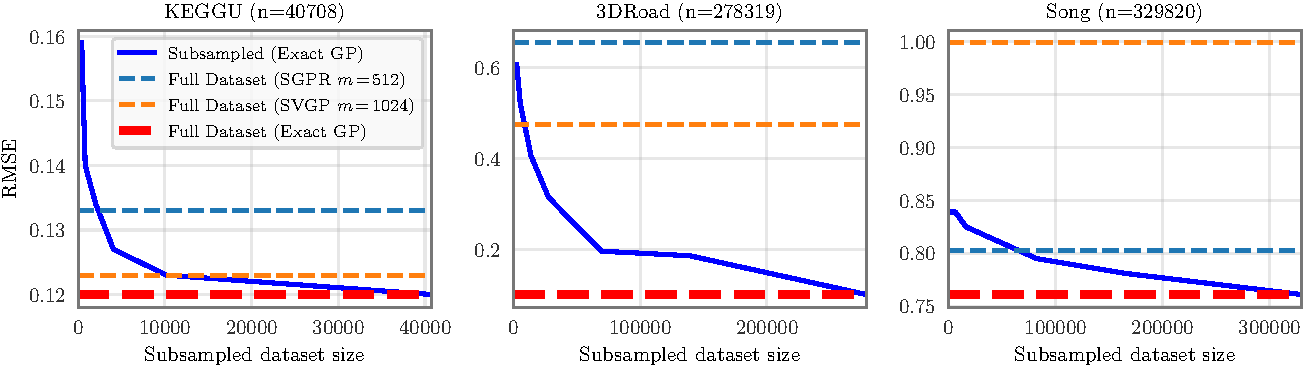
\includegraphics[width=0.7\linewidth]{figures/subsampling.pdf}
  \caption[Effect of training set subsampling on exact GP performance.]{
    Effect of training set subsampling on exact GP performance, as measured by test set RMSE (lower is better).
    Subsampled exact GPs outperform approximate GPs, even when only quarter of the training set is used.
    Exact GP error continues to decrease as data is added.
  }
  \label{fig:subsampling_results}
\end{figure}

\paragraph{Do GPs need the entire dataset?}
As a non-parametric model, Gaussian processes naturally adapt to the amount of training data available.
\cref{fig:subsampling_results} shows an increase in accuracy as we increase the amount of training data on the KEGGU, 3DRoad, and Song datasets.
For each dataset, we subsample a fraction of the training data and plot the resulting test set RMSE as a function of training set size.
As expected, the error decreases monotonically as we increase the subsample size.
\cref{fig:subsampling_results} also shows the performance of exact GPs, SGPR, and SVGP trained on the entire dataset.
Strikingly, in all three cases, \textit{an exact GP with less than a quarter of the training data outperforms approximate GPs trained on the entire training set}.
Test error continues to decrease with the addition of training data.

\begin{figure}[!t]
  \centering
  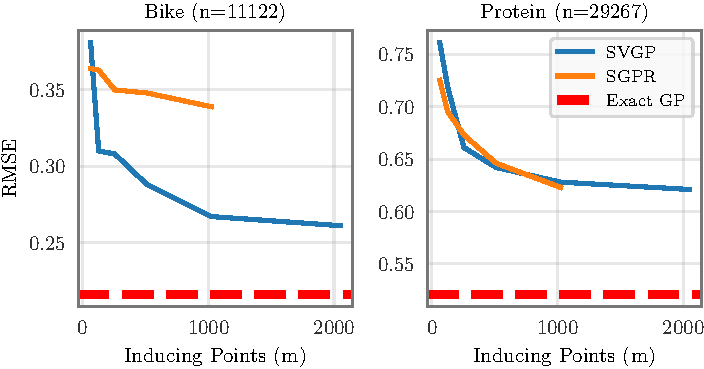
\includegraphics[width=0.7\linewidth]{figures/inducing_points.pdf}
  \caption[Error of approximate GP methods as a function of the number of inducing points.]{
    Error of SVGP and SGPR methods as a function of the number of inducing points ($M$).
    Both methods scale cubically with $M$.
    We are unable to run SGPR with more than $1,\!024$ inducing points on a single GPU.
    Exact GPs have lower error than both methods.
  }
  \label{fig:num_inducing_points}
\end{figure}

\paragraph{Would more inducing points help?}
The results in \cref{tab:large_exact_gp_results} naturally raise the question: ``can approximate models with more inducing points recover the performance of exact methods?''
In \cref{fig:num_inducing_points}, we plot test set RMSE on two datasets, Bike and Protein, as a function of the number of inducing points.
We note that in theory the performance of SVGP and SGPR should match exact GPs as $M \rightarrow N$ \cite{titsias2009variational,hensman2013gaussian}.
In practice however, the test RMSE of SGPR and SVGP remains well above exact GPs, and adding more inducing points has diminishing returns.
We note that using $M$ inducing points introduces a $M \times M$ matrix and a $\bigo{NM^2 + M^3}$ time complexity which makes it difficult to train SGPR with $M \gg 1024$ inducing points.
It is possible to combine partitioned kernel MVMs with inducing-point methods to utilize even larger values of $M$.
However, as \cref{fig:num_inducing_points} and \cref{tab:large_exact_gp_results} show, it may be preferable to use the extra computational resources to train an exact GP on more data rather than to train an approximate GP with more inducing points.
